\documentclass[english]{article}

\usepackage{babel}
\usepackage{graphicx}
\usepackage{times}
\usepackage{pifont}
\usepackage[margin=1in]{geometry}
\usepackage{eurosym}
\usepackage{fancyhdr}
\usepackage[hidelinks]{hyperref}
\usepackage{pdfpages}
\usepackage{enumitem}

\pagestyle{fancy}
\fancyhf{}


%HEADER
%**************************************************************************************
\pagestyle{fancy}
\fancyhf{}
%**************************************************************************************
\lhead{Thesis}		 	 
\rhead{Thesis Plan} 
\lfoot{EFA12SF}
\cfoot{\thepage}
\rfoot{Alexey Tukalo}
%**************************************************************************************

\date{}
\setlength\parindent{0pt}

\begin{document}

\title{\vspace{2in}Thesis Plan\\
\small for Bachelor Thesis\\
\vspace{0.5in}
\includegraphics{savonia.jpg}}

\nopagebreak
\maketitle


\vspace{3in}

\author{
\begin{flushright}
Alexey Tukalo,\\
EFA12SF,\\
Information Technology,\\
Savonia University of Applied Sciences
\end{flushright}
}

\date{\today}
\thispagestyle{empty}
\newpage
\setcounter{page}{1}
%MAIN CONTENT ******************************************************************************************************************

\section{Introdaction}

Volume rendering is a well known concept as computer graphics, the main theoretical base was developed at 80s and early 90s. Nowadays an ordinary work station gives as an opportunity to render an interactive volume scenes and as result the topic is experiencing a significant revival. The technology is used for visualisation of medical studies, scientific data collected by different types of sensors and physical models for particles, fluids and gases.\\

I made myself familiar with a concept of volume rendering during my internship at Karlsruhe Institute of Technology(KIT), there I worked on modification of Tomoraycaster 2 to give it an opportunity to render multimodal volume data.\\

I am going to implement an engine for volume rendering with DirectX in C\#, the engine will become a part of LightningChart. LightningChart is a proprietary library for visualisation of scientific data developed by Arction Oy. Arction wants to add volume rendering possibilities to their product, but an existing solution does not suit them well, because they need to have very deep integration with their current engine and they want to keep their source code as independent as it is possible.

\section{Theory base}

As I already noticed, the theoretical base for the volume rendering was developed more than 20 years ago. The idea started from the rendering equation simultaneously derived by David Immel and James Kajiya in 1986.

There are four main volume rendering technics:
\begin{itemize}
\item Volume ray casting
\item Splatting
\item Shear warp
\item Texture-based volume rendering
\end{itemize}

I am going to start the development from an implementation of the most basic Ray Casting algorithm. The Ray Casting also called image-ordered volume rendering. Basically, it shoots rays from every pixel in the screen and samples the data from the volume in according with so called ray function. The ray function is an equation which determines how the volume would be sampled.\\

The technique has two main advantages:
\begin{itemize}
\item Very high quality with very low amount of artifacts
\item Number of various ray functions gives as an extra flexibility
\end{itemize}

But the Ray Casting has a very big disadvantages, it contains a lot of interpolations for the calculations of hit points of the ray, it makes the algorithm relatively slow.\\

So, I am going to speed the engine up by moving the implementation to the Shear warp realisation. Basically the algorithm is an optimisation of ray casting approach which is created to avoid any kind of calculations related with an interpolation at the sampling stage. It is realised by an additional preprocessing stage called Shear. The stage contributes some artifacts which are reduced at the last step of rendering called Warp. In other words, Shear-warp is realisation of Volume Ray Casting with two additional pre and postprocessing steps.\\

\section{Objectives and results} 

The final result of the project is realisation of an interactive volume rendering engine integrated into two versions of LightningChart(DX9 and DX11) which will became private property of Action Oy.

\section{Implementation}
The engine has to be integrated inside LightningChart, so on the one hand it restricts me to use C\#, HLSL and DirectX as my main tools. In the other hand I can get significant profit from the features already implemented inside the library, for example it will help me to implement rotation of the object, mouse interaction detection and so on.\\

I will be responsible for the development of the entire engine and visualisation based on the engine. The visualisation would be an example of the main possibilities which the engine will provide to the LightningChart. It will give us an opportunity to test and verify the software quality. The project will be implemented under mentoring of Mr. Pasi Tuominen\footnote{CEO of Arction Oy}, he will guide me in terms of source code organisation and evaluation of the final solution.\\

I broke the development to the several steps:
\begin{enumerate}
\item Create testing application with a cube which would represent the inner boundaries of the volume. 
\item Implement the most basic shader and new type of objects which will be rendering with this shader.
\item Read the volume data as set of textures.
\item Preprocess the texture to fit the hardware. 
\item Implement the most basic Volume Ray Casting. 
\item Implement a mouse interactions with the volume.
\item Optimize the volume rendering: 
\begin{enumerate}
\item Add Shear and Warp steps to the Ray Caster 
\item Add spatial structure optimization
\end{enumerate}
\item Implement rotation.
\item Implement lightning effects. 
\item Port the solution for an other version of LightningChart.
\end{enumerate}

\section{Resources}
All the resources needed for the development are provided by Arction Oy:
\begin{itemize}
\item The workstation with Windows
\item Visual Studio and other software
\item Development version of LightningChart
\end{itemize}

The main part of the work would be made by myself, so any addition human resources are not needed.
In according with my calculations the project will took me from 240 to 360 hours, and it will cost Arction from 1500 to 2000 \euro.
\section{Risk}

The project has very low risks, because I am going to use well known techniques based on fundamental researches and my implementation is going to be made on the highly reliable technologies widely used in the market. The solution will become a part of the LightningChart to give current Arction's customers new possibilities and attract new ones interested in the feature.\\

The source code created during the project will become private property of Arction Oy.

\section{Report documentation}
Preliminary table of contents and a documentation plan of the final thesis:
\begin{enumerate}
\item Introduction to Volume Rendering 
\begin{enumerate}[label*=\arabic*] 
\item Motivation \item Introduction to LightningChart 
\item Volume Rendering Algorithms
 \end{enumerate}
\item Implementation of the Volume Rendering 
\begin{enumerate}[label*=\arabic*] 
\item Implementation of Volume Ray Casting 
\item Optimization of the engine 
\item Advantages of Shear Warp 
\end{enumerate}
\item Results
 \begin{enumerate}[label*=\arabic*] 
\item Evaluation 
\item Discussion 
\item Conclusion 
\end{enumerate}
\item References
\end{enumerate}

Arction does not request any additional reports. Results of the project will be presented to the University on the seminar presentation.
\section{Appendix}
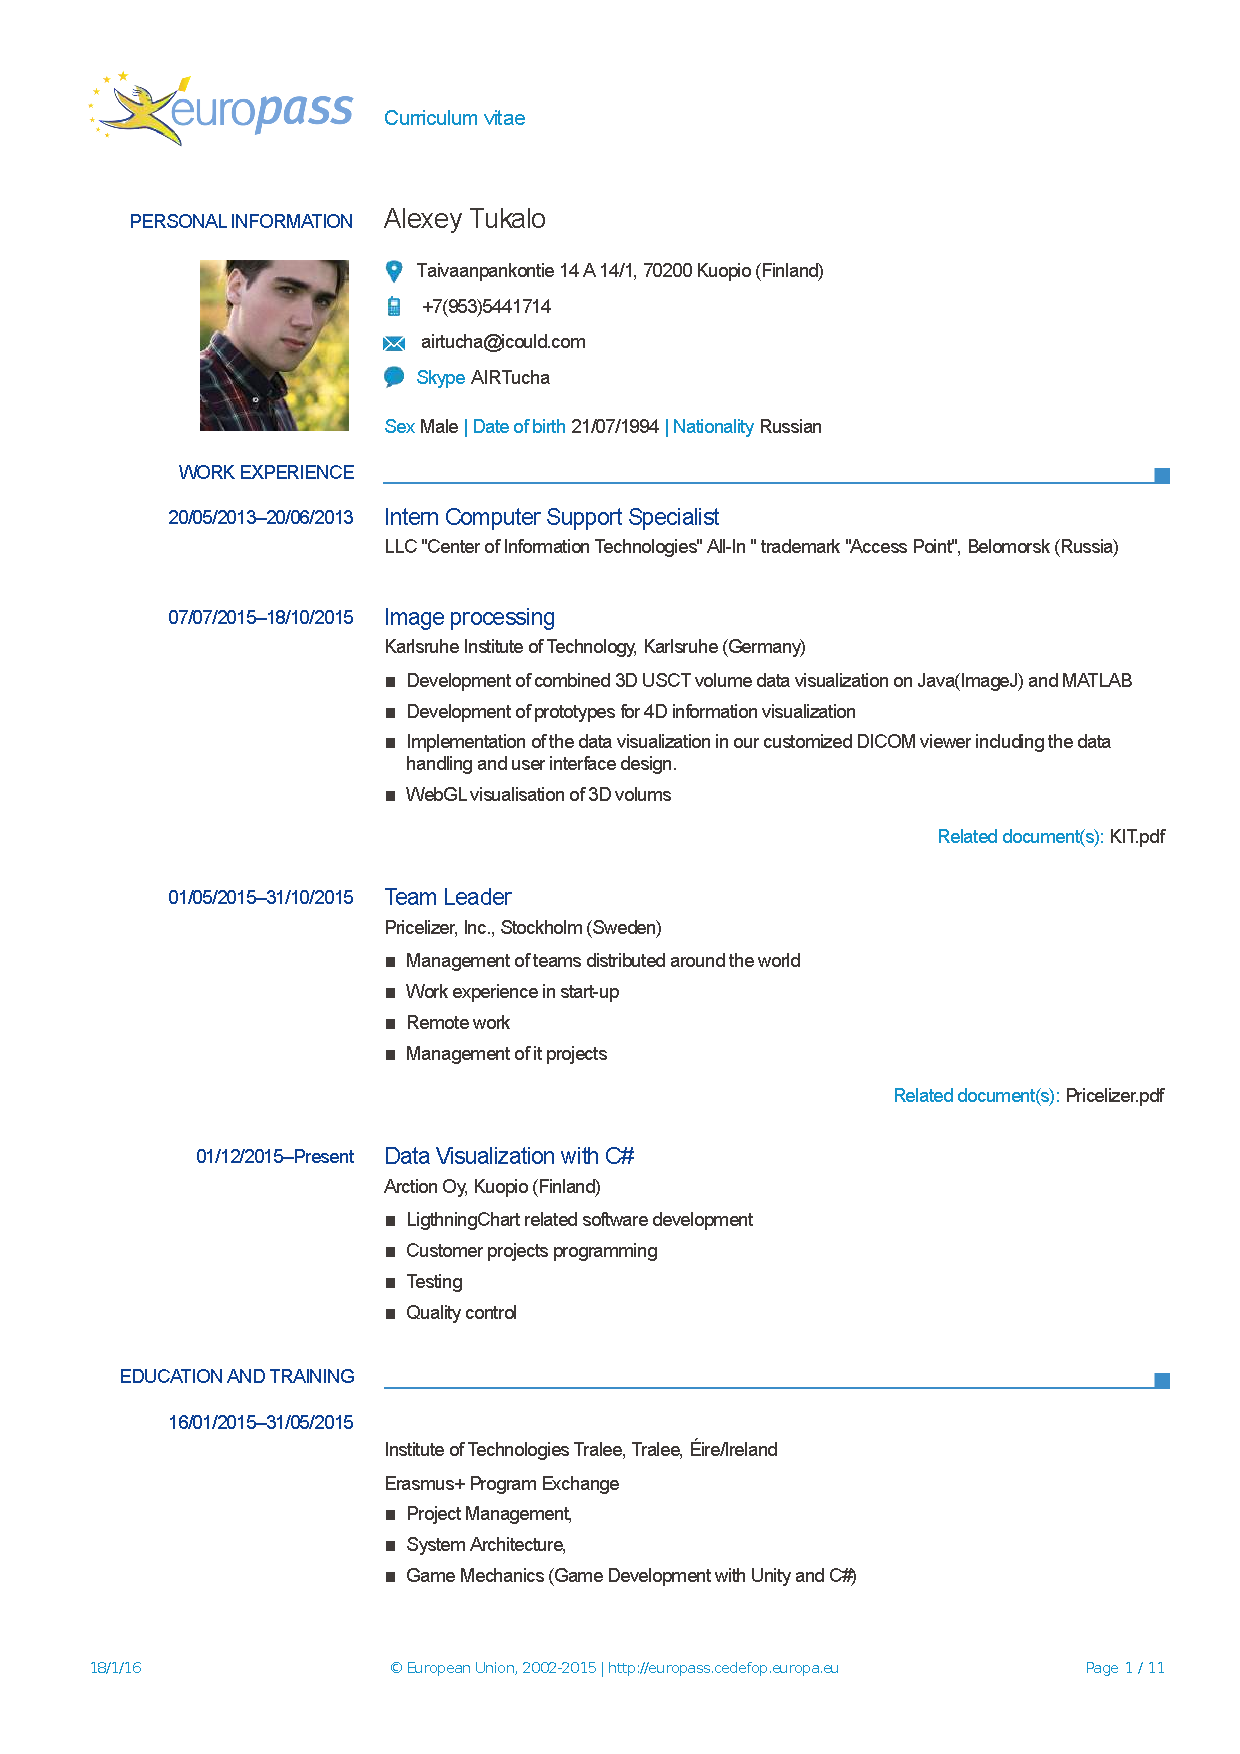
\includepdf[pages=-]{thesis/cv.pdf}


\end{document}
